\chapter{Forces}
\label{chap:forces}
\section{Introduction}

Forces are an essential element in the study of physics. The concept of force is familiar: effects of forces such as friction and the gravitational force on the human body are part of everyday experience. Thanks to Isaac Newton who proposed his 3 laws of motion, forces are both physically and mathematically well defined; forces can be measured, combined, and evaluated in exact ways. This laboratory experiment  is intended to demonstrate a few of the many examples of commonly encounterd forces discussed in the lecture course and how Newton's laws can be used to analyze their behavior. \myskip

The objective of this lab is to  illustrate the properties of several forces and how we can observe them. First, we deal with the vector nature of forces and how static equilibrium requires that the sum of forces on single object must be zero. The forces arise from the gravitational attraction to the earth (weight) of objects, which are transmitted to a point through string tension.\footnote{See Chapters 5 and 12 of \emph{Fundamentals of Physics} by Halliday, Resnick \& Walker.} \myskip

Next, we work with the force arising by stretching or contracting a spring. This kind of force has more general applications than springs, in that the "elastic'' nature of collisions (like a tennis ball bouncing on the floor) arises from spring-like forces. You will measure the quantitative relationship between the force applied to a spring and the subsequent displacement from equilibrium.\footnote{See Section 7-7 of Halliday, Resnick \& Walker.} \myskip

Finally, we deal with a dynamic system where we use computer data acquisition to measure the acceleration caused by gravitational and frictional forces acting on a cart traveling down an inclined plane. \myskip

\section{Theory}

\subsection{Vector Representation of Forces}

In the first part of the experiment, we measure three vector forces and show that when the system is stationary, the sum of all forces is zero. Vectors have both length \emph{and} direction, and can be represented graphically by an arrow -- the length corresponds to the magnitude of the vector, while the direction (from tail to head) corresponds to the direction of the vector. To add two vectors graphically, simply place the tail of one vector at the head of the other. Then start from the same origin and attach the two vectors in the reverse order, we must arrive at the same final point. From the parallelogram formed by this procedure, the arrow along the main diagonal represents the sum of the two vectors (The other diagonal is the difference of the two vectors). See figure \ref{fig:graph} for an example of graphical addition of two vectors.
\begin{figure}[h]
    \begin{center}
        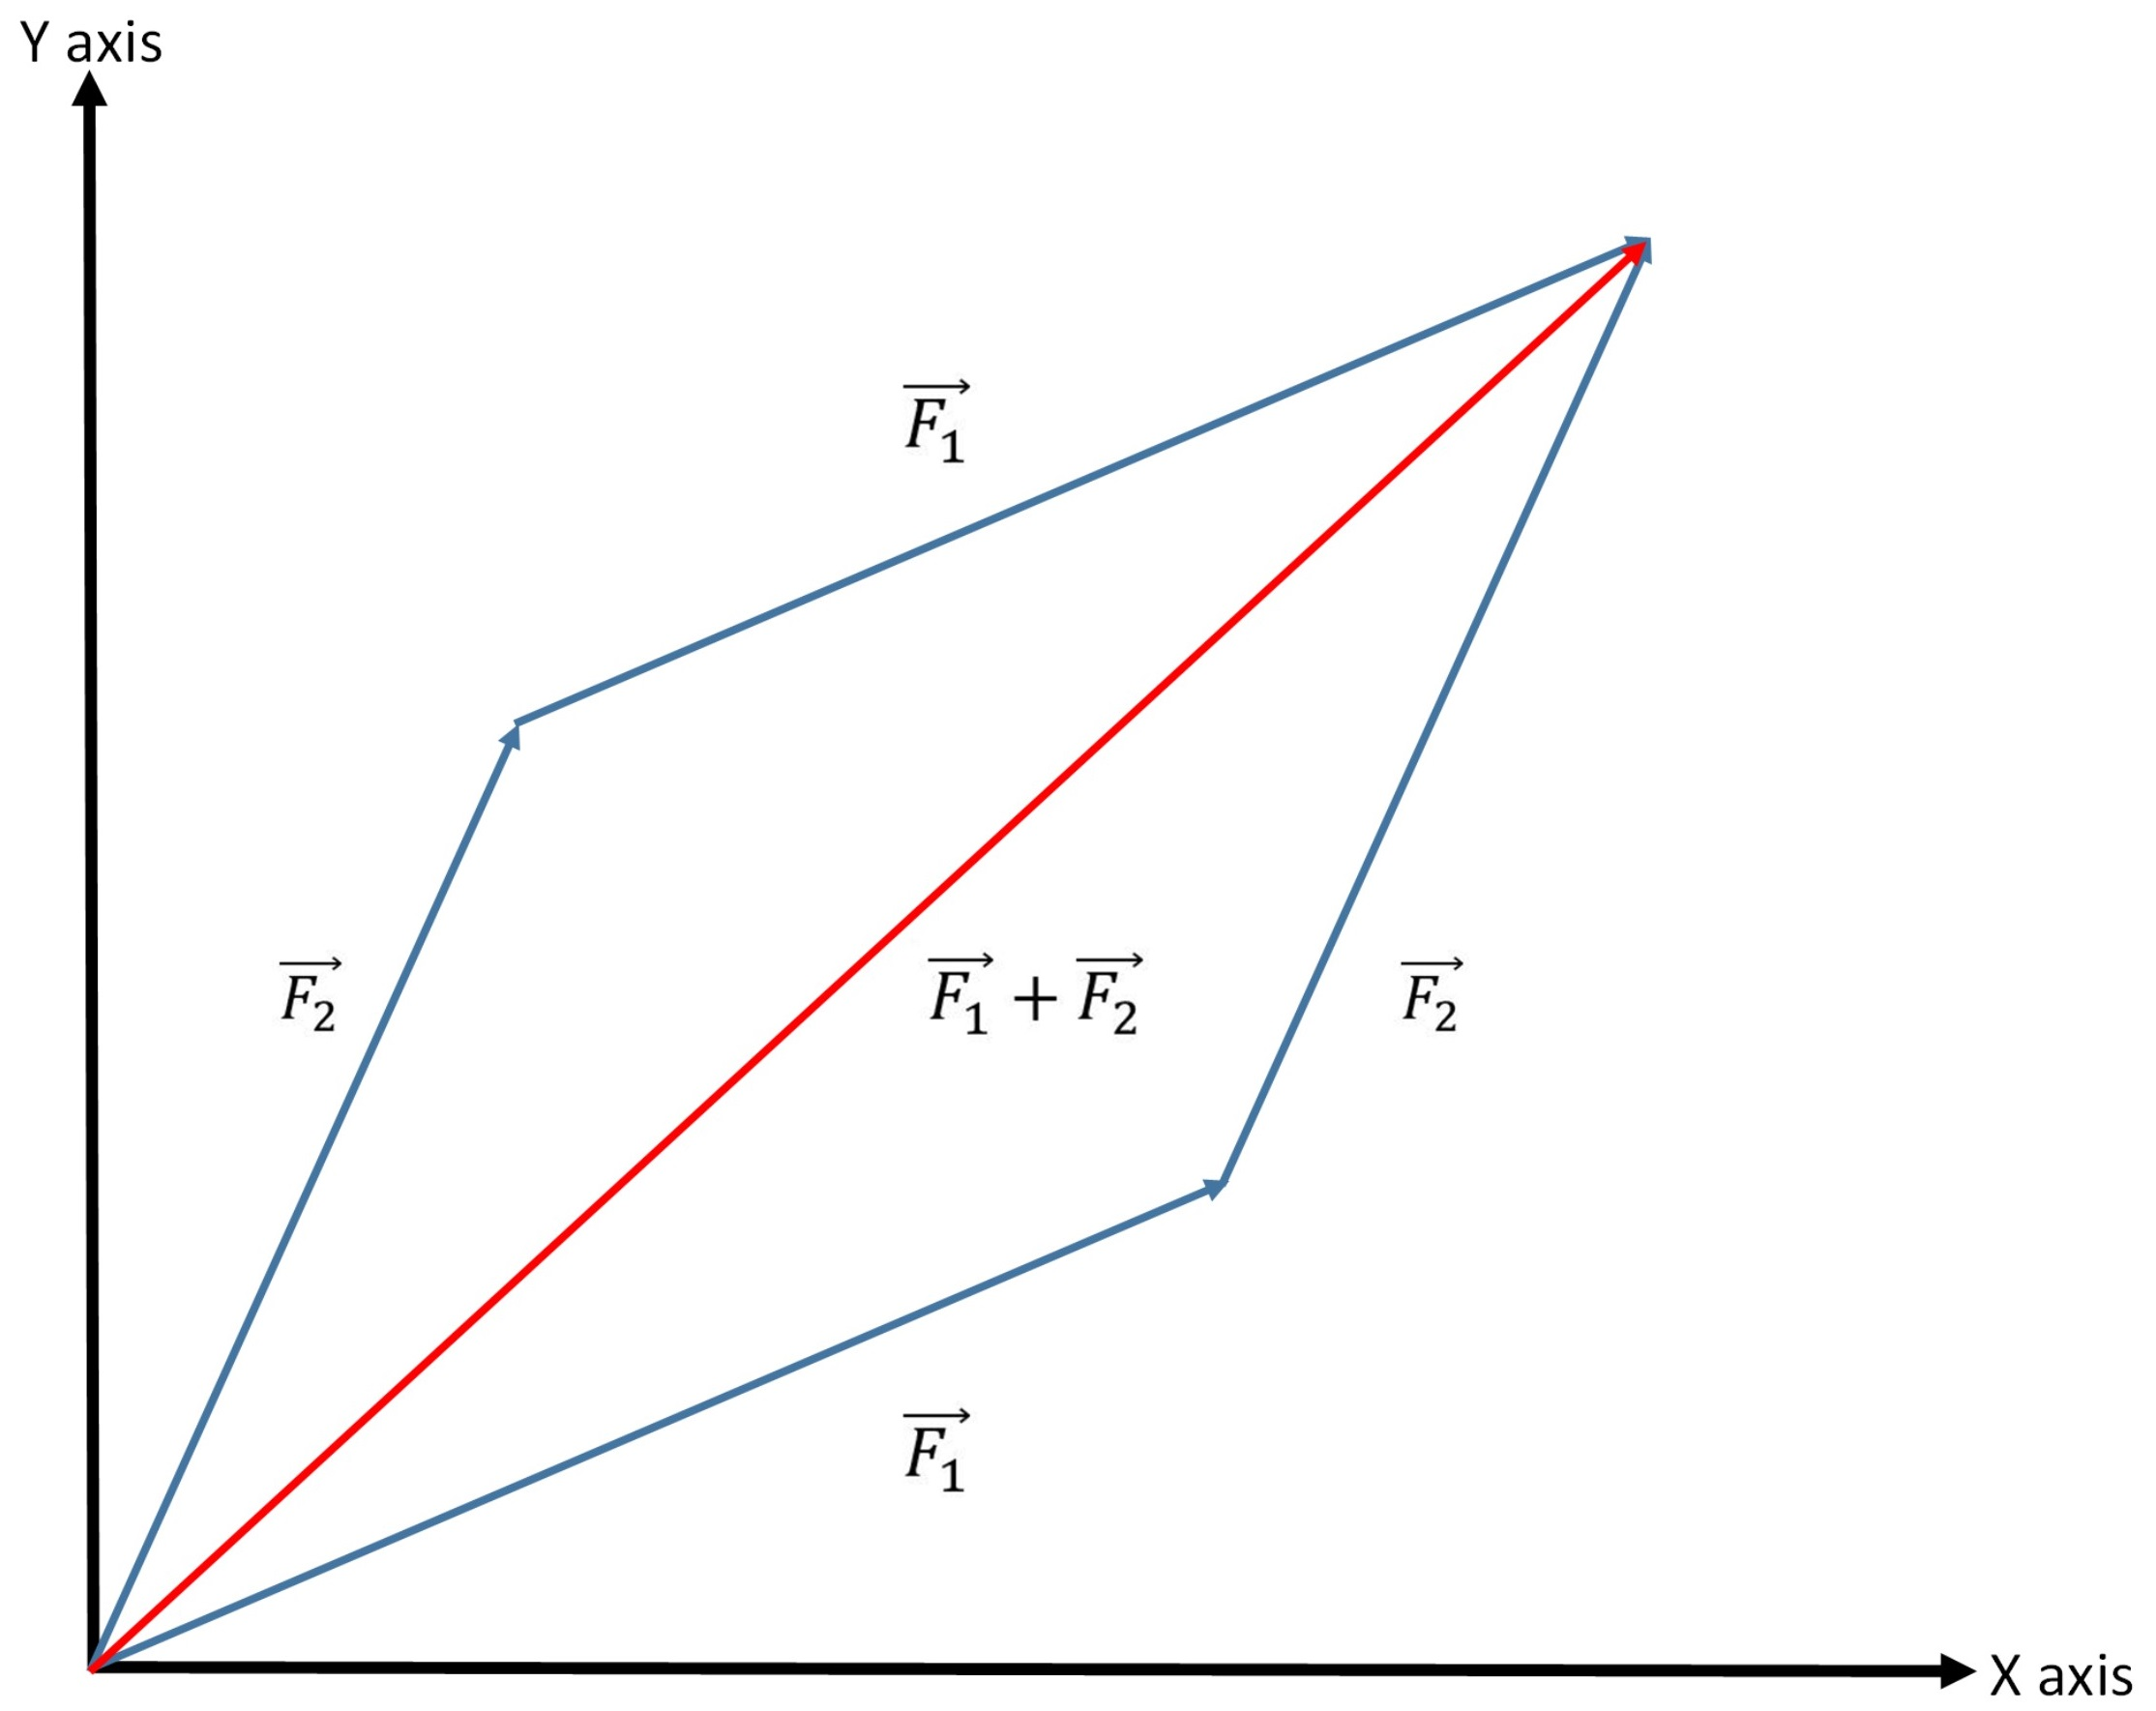
\includegraphics[width=0.7\textwidth]{./Exp3/pic/image11.jpg}
    \end{center}
    \caption{An example of graphical addition of two force vectors $F_1$ and $F_2$.}
    \label{fig:graph}
\end{figure}

Vectors can also be added algebraically. Vectors are typically described in cartesian coordinates, where the $x$, $y$, and $z$ components of the vectors are identified, e.g.\ $\vec u = (u_x,u_y,u_z)$. When adding multiple vectors, you must add all vectors in the same coordinate system (i.e. the x component of one vector must point in the same direction as the x component of the other vector, etc...). For example, if we have two vectors described in cartesian coordinates, ($\vec u = (u_x,u_y,u_z)$ and $\vec v = (v_x,v_y,v_z)$), the components of the sum, or resultant, vector are $\vec u+\vec v = (u_x + v_x, u_y + v_y, u_z + v_z)$.\myskip

\begin{figure}[h]
    \begin{center}
        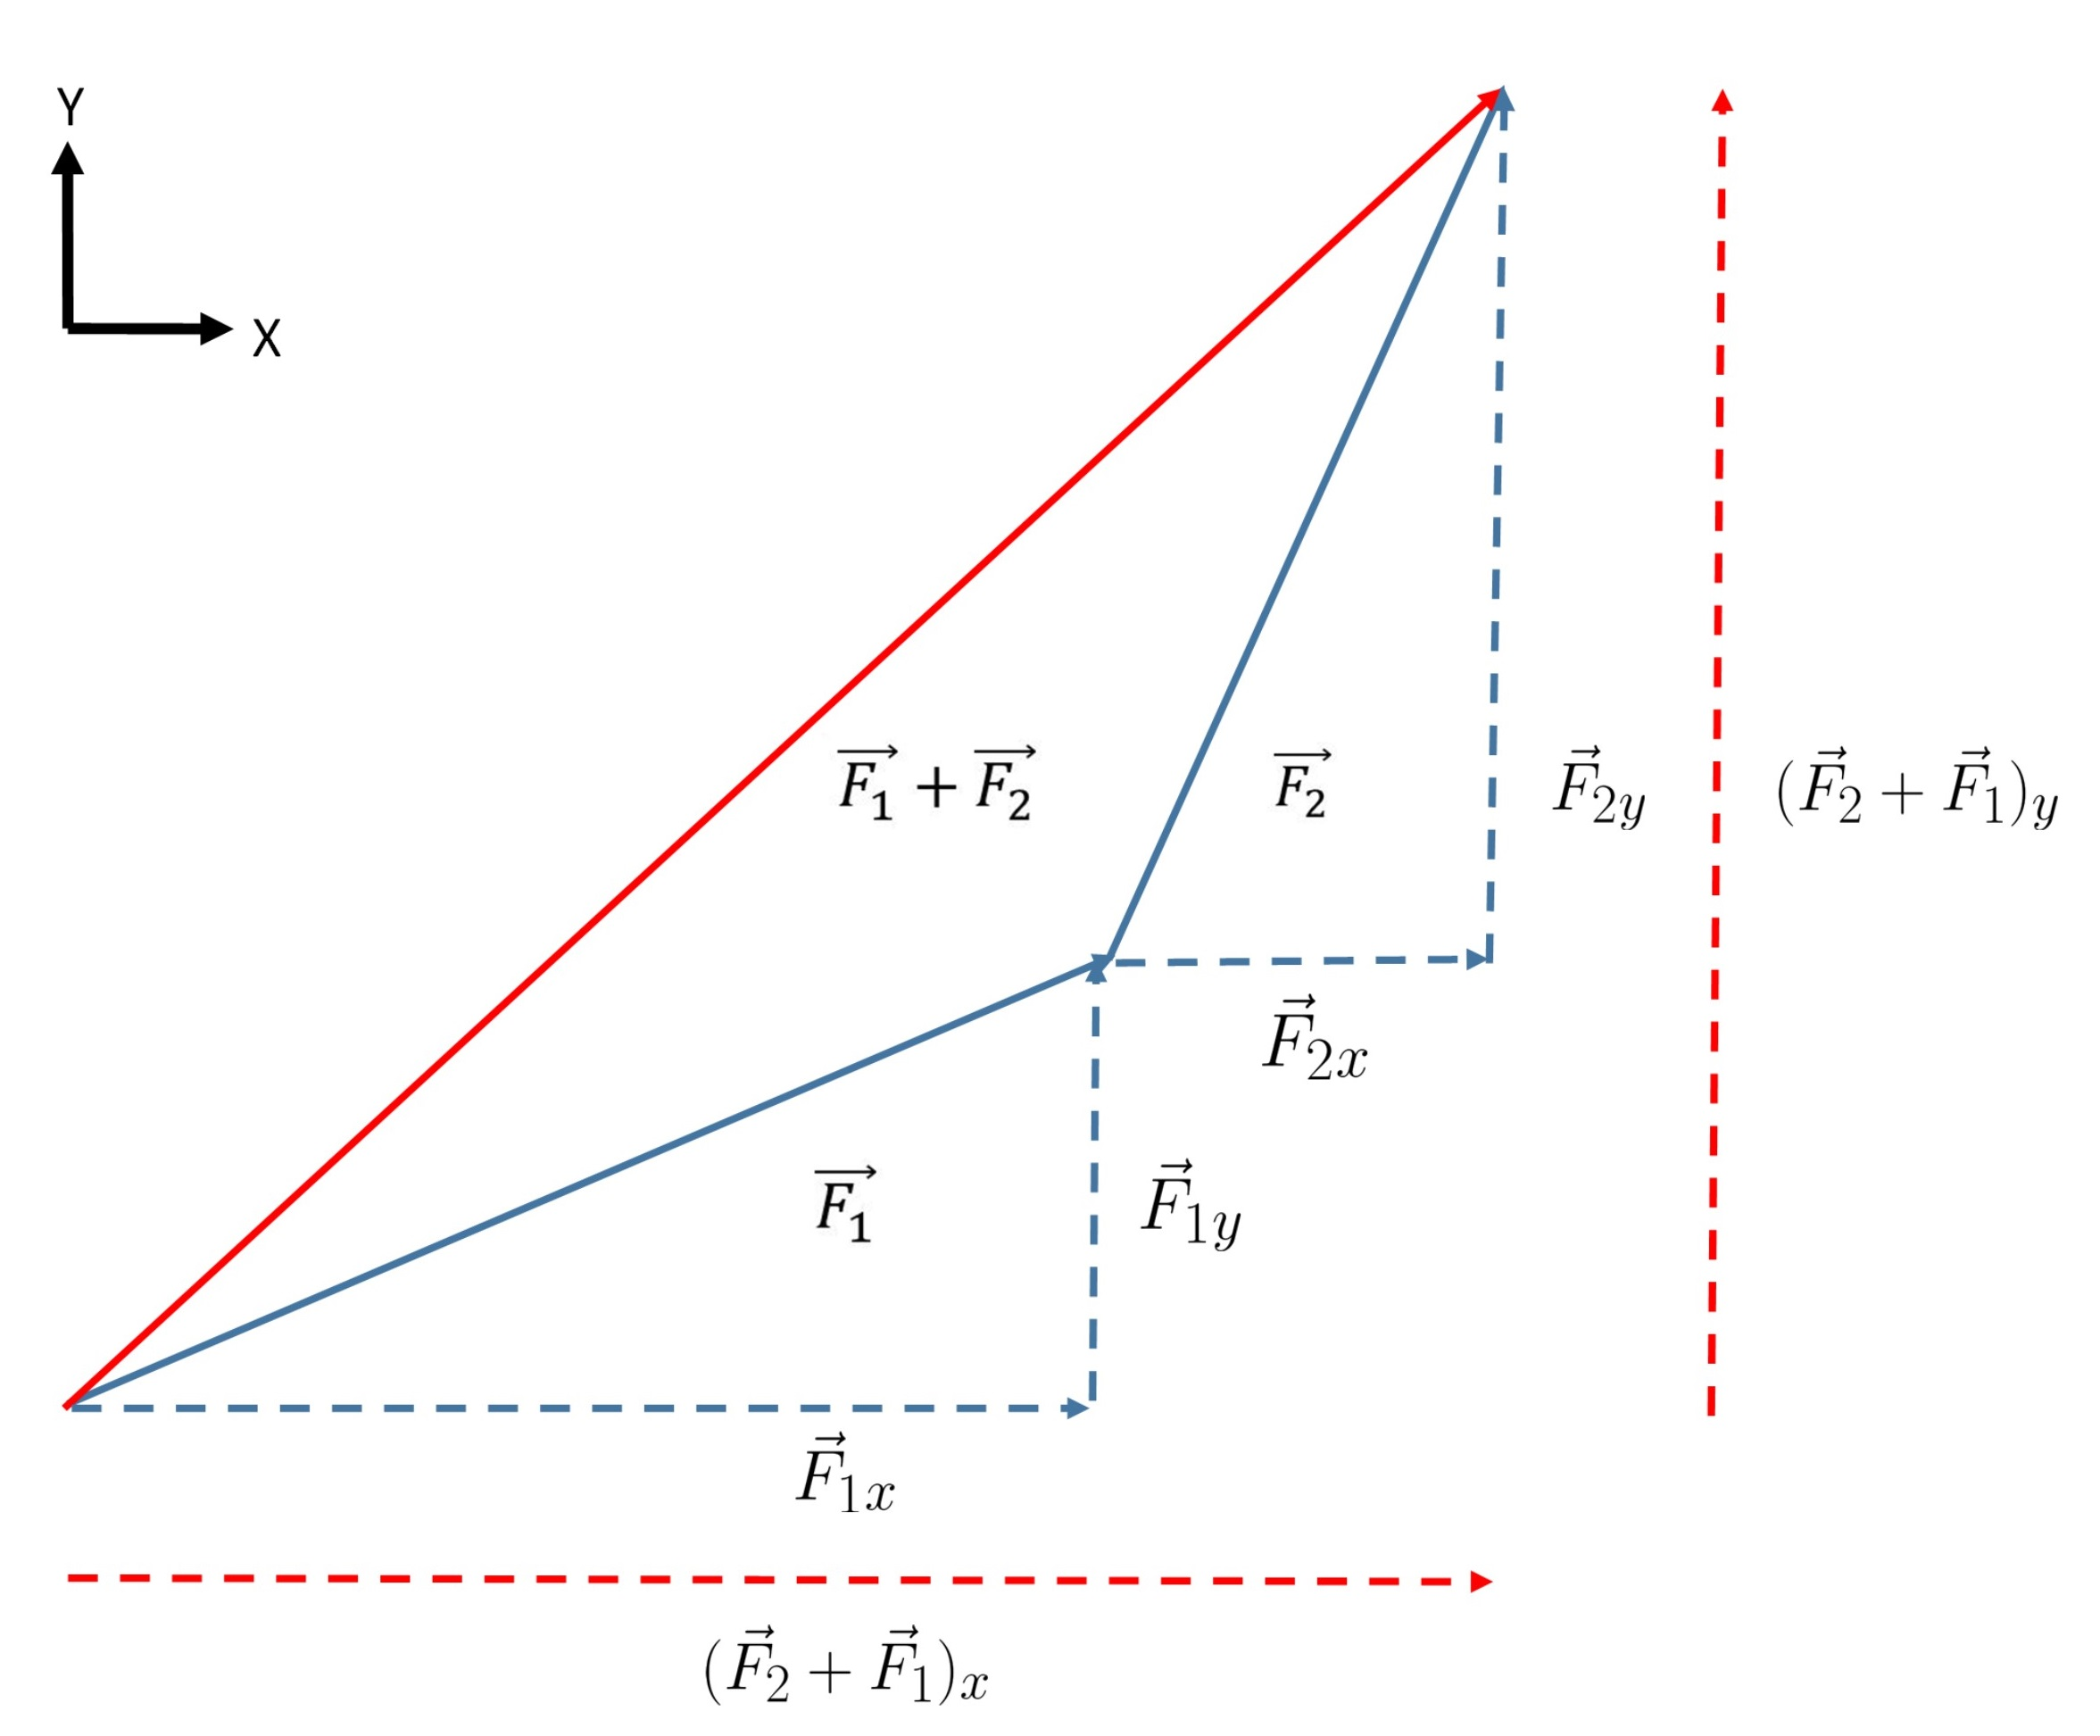
\includegraphics[width=0.8\textwidth, height=0.6\textwidth]{./Exp3/pic/image12.jpg}
    \end{center}
    \caption{An example of splitting up force vectors into components to add them algebraically.}
    \label{fig:add}
\end{figure}

In order to add vectors algebraically, we take advantage of the fact that vectors can be split into components at right angles to each other (in the example above, we split vectors into $x$, $y$, and $z$ components). This is an important tool we use in physics repeatedly. You may choose, for the convenience of doing the problem, your $x$, $y$, and $z$ axes. There is usually a favorable choice of axes in which the problem can be described most easily. See figure \ref{fig:add} for an example of splitting up the force vectors in figure \ref{fig:graph} into components and adding them to find the components of the resultant vector.

\subsubsection{Parallax}

In the first part of this lab, we must draw images on paper of strings located some nonzero distance above the paper. It will at first appear that there are many different possibilities of where to draw the images of the strings. If you draw lines on the sheet that seem directly below the strings when your head is in a given position, if you move your head a few centimeters left or right you will see that the lines are no longer covered by the strings. This effect, in which a closer object (here the string) seems to move relative to a distant background (here the sheet on which you draw the line) is called \emph{parallax}. We will see effects of parallax several times during these labs, so it is important to learn how to handle it. \myskip

Where should the lines be drawn?  A unique prescription for where to place the lines is provided by the instruction to \emph{always look straight down on the string}. Now we must determine how we know when we are looking straight down on the string. Use a small mirror and place the mirror on the sheet directly under the string. Both the string and the image of the string in the mirror are visible. As your head moves left and right, the mirror image of the string moves relative to the string. When your head is located so that the string and its mirror image exactly overlap, \emph{you are looking straight down}. Make two small marks beside the mirror where the image of the string enters and leaves the mirror. Then, remove the mirror and draw a line through the two points on the paper with a ruler. This line is the correct image of the string.

\subsection{Springs}

Ideal springs turn out to have a very simple relation between the force $F$ applied to them and the distance $s$ they are stretched from equilibrium. This \emph{linear} relationship, called ``Hooke's Law',' is expressed by:
\begin{equation}
  \vec  F = -k \vec s
\end{equation}
where $k$ is known as the ``spring constant''\footnote{Note that this denotes the force applied \emph{to} the spring, not the force from the spring due to Newton's 3rd law}. It is a quantity characteristic of each individual spring and its value depends only on the properties of that spring (such as elasticity of the metal, number of coils per length, etc...). In this lab, we will measure the forces necessary to stretch a spring different distances from equilibrium, and from these we will determine the spring constant of the spring.


\subsection{Inclined Plane}
\begin{figure}[h]
    \begin{center}
        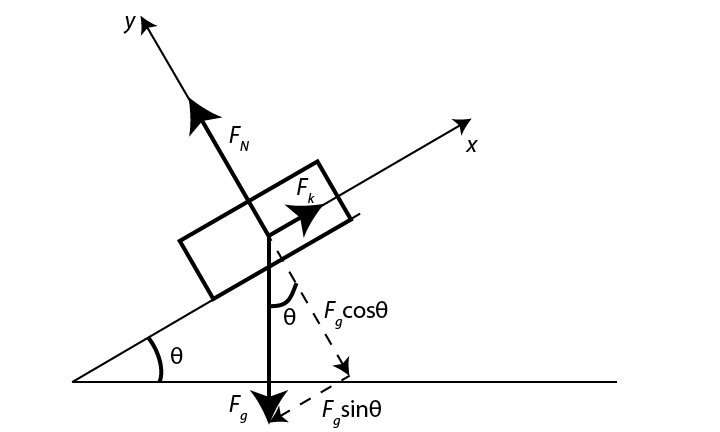
\includegraphics[width=0.8\textwidth]{./Exp3/pic/image16.png}
    \end{center}
    \caption{An inclined plane with kinetic friction.}
    \label{fig:plane}
\end{figure}
In the last part of this lab, we will be looking at the prototypical dynamic system in motion: the inclined plane.  When a block slides down an incline there are typically three forces at play: the gravitational attraction to the center of the earth, $F_\text{g}$; the normal force that prevents the block from going through the inclined plane, $F_\text{N}$; and the kinetic frictional force that slows the descent of the block, $F_\text{k}$.  Since the net force on the block must be parallel to the surface, using a tilted coordinate system, as in Figure \ref{fig:plane}, makes it clear that the net force is the following:
\begin{gather}
\vec F_{\text{net}} = - F_{\text{g}} \sin(\theta) \hat x + F_{\text{k}} \hat x = \left ( \mu_k F_N-F_{\text{g}} \sin(\theta)\right ) \hat x
\end{gather}
Since the normal force, $\vec F_\text{N} = F_\text{g} \cos(\theta) \hat y$ and $\vec F_\text{g} = -m g \hat y$ we can derive the following:

\begin{equation}
\vec F_{\text{net}} = \left ( mg \sin(\theta) - \mu_\text{k} m g \cos(\theta) \right ) \hat x= m\vec a
\end{equation}
\noindent Consequently, the acceleration of the block will only depend on the angle of the incline and coefficient of kinetic friction, $\mu_k$. If we solve for $\mu_k$ we get the following relationship:

\begin{equation}
\mu_\text{k} = \tan(\theta)-\frac{a}{g \cos(\theta)}
\end{equation}

\section{Procedure}

\subsection{Addition of Forces}

In the first part of the experiment, we deal with three different forces due to hanging masses. The force due to an unknown weight will be exactly balanced by two known forces. We will determine the unknown mass with uncertainty using the graphical addition of vectors and Newton's second law for a stationary objects. \begin{figure}[h]
    \begin{center}
        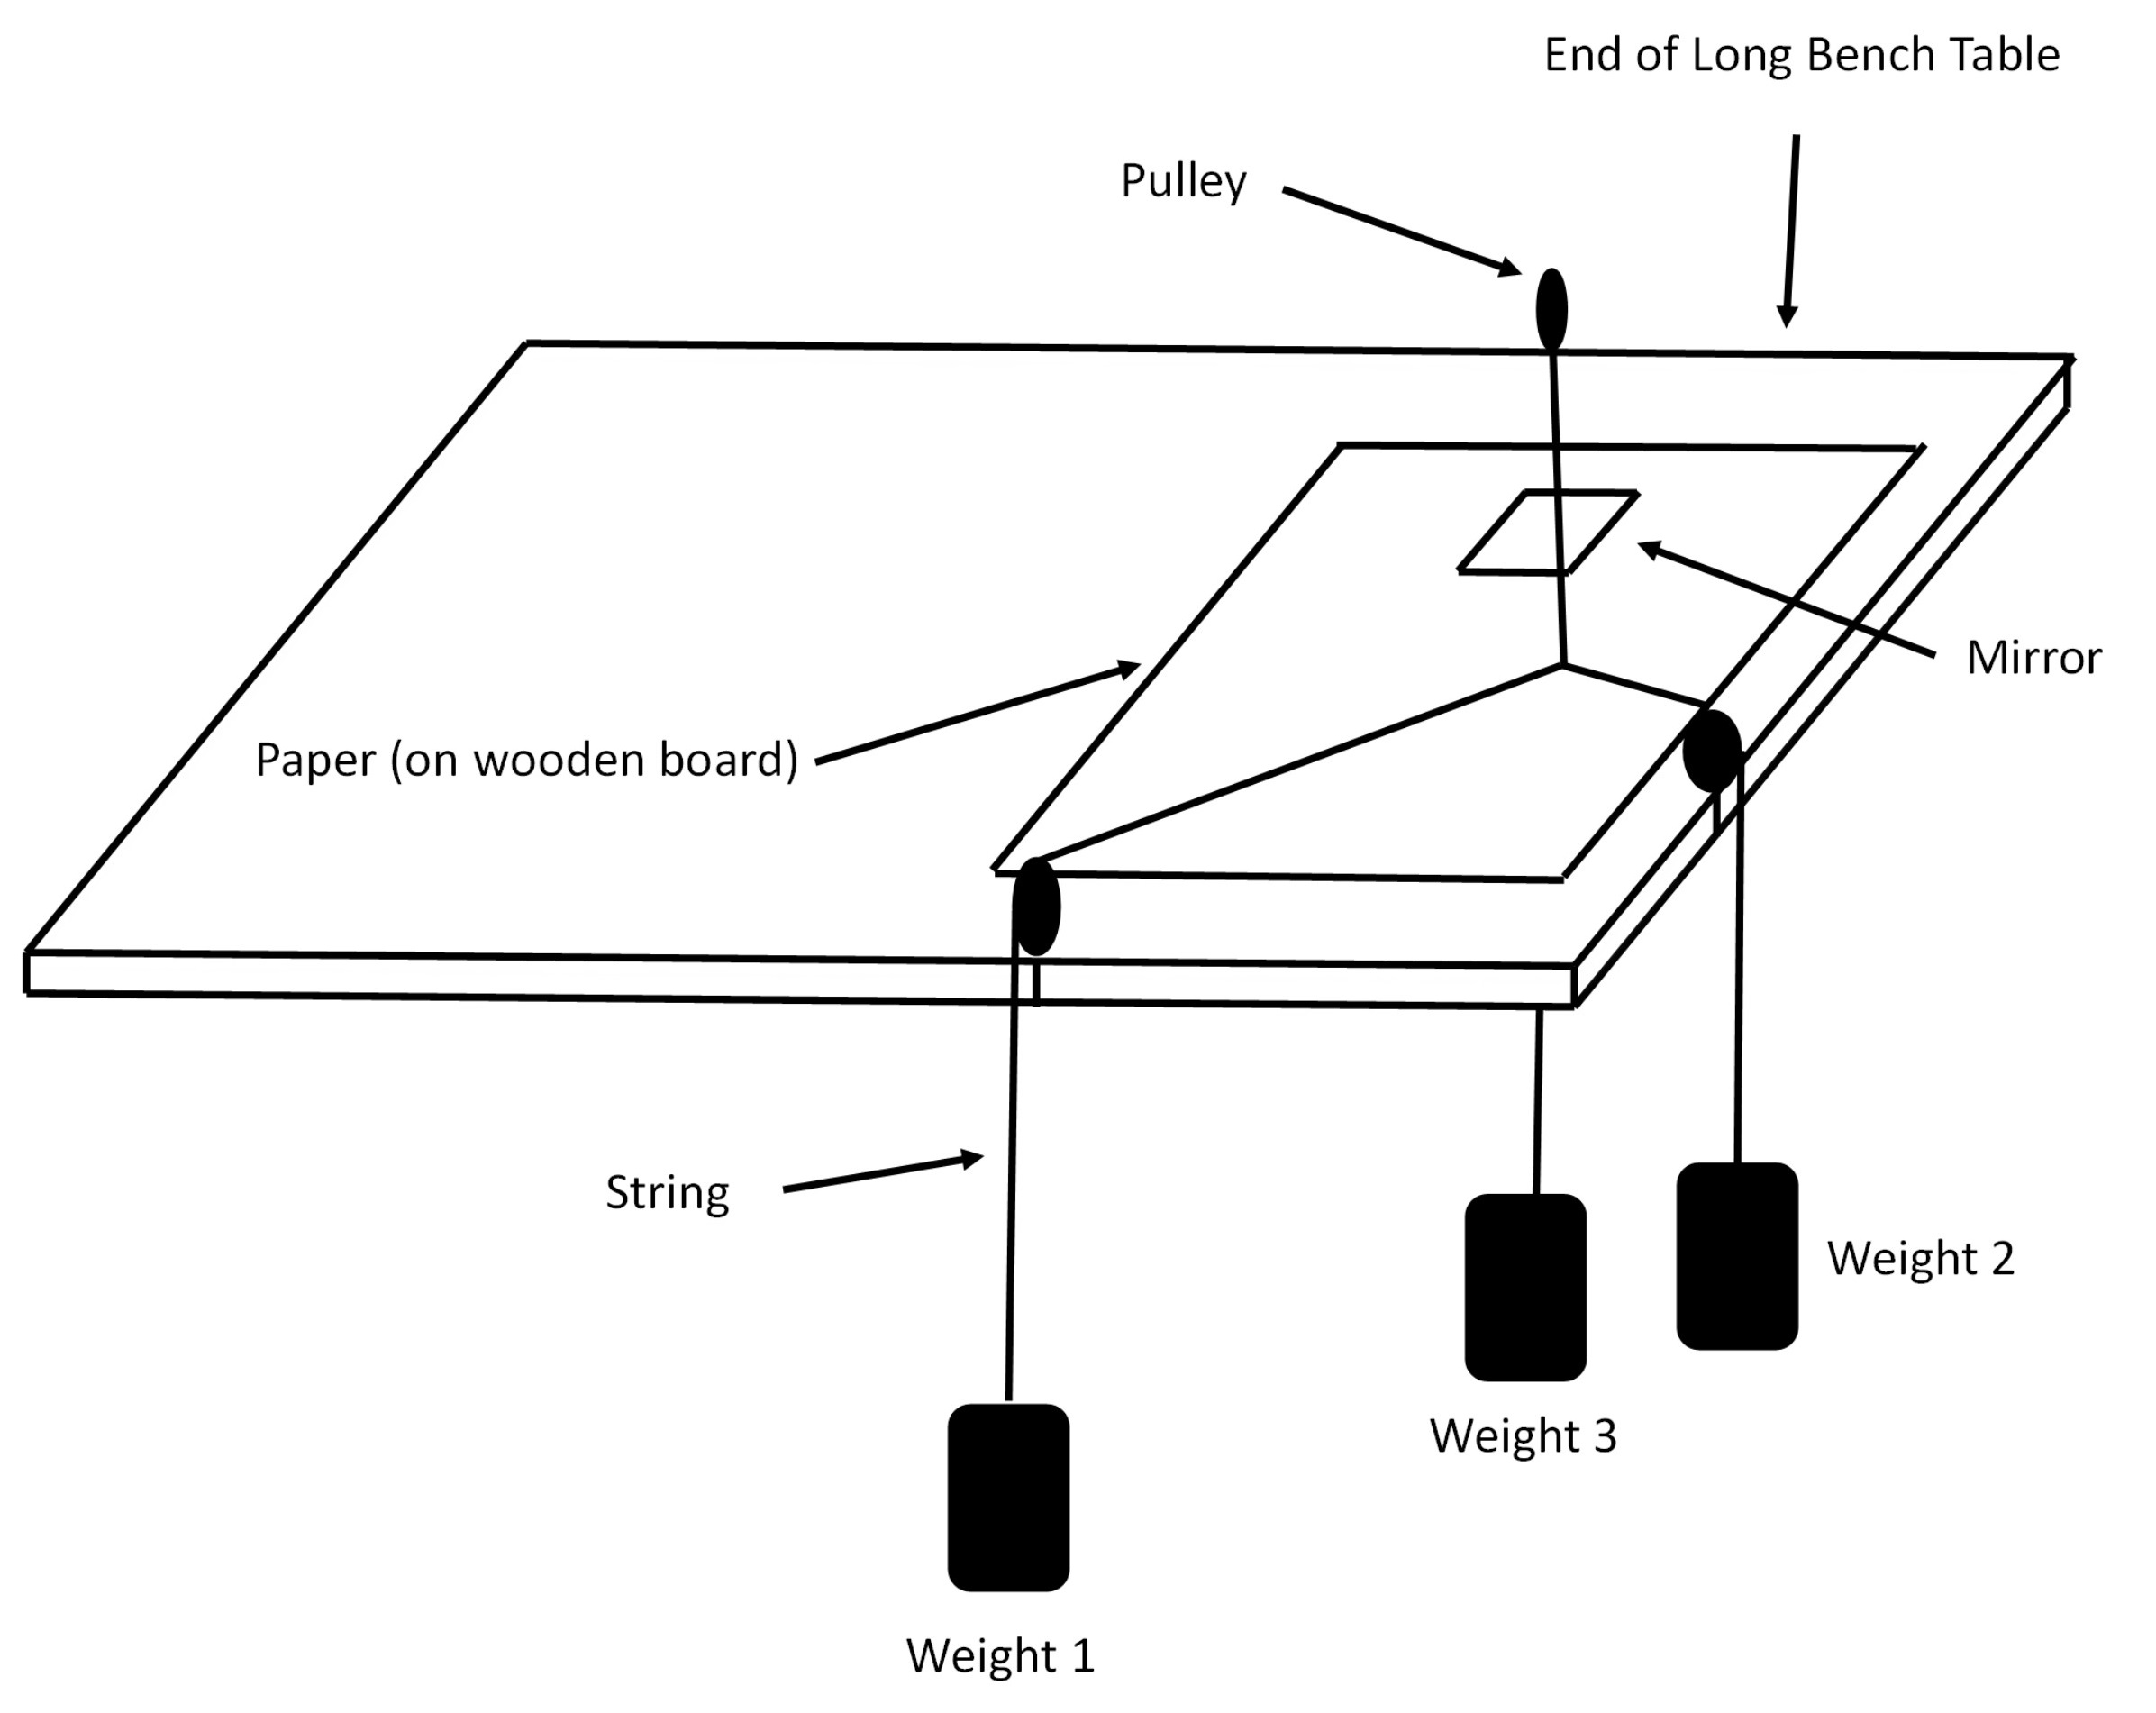
\includegraphics[width=0.8\textwidth]{./Exp3/pic/image14.jpg}
    \end{center}
    \caption{Experimental Setup}
    \label{fig:setup}
\end{figure}

The equipment includes a wooden board to which three pulleys are clamped. Over each pulley, we place a string with a weight (making sure the string doesn't slip off the pulley). Choose two different known weights and attach them to two of the strings (you might begin with a $100\,\mathrm{g}$ and $150\,\mathrm{g}$ weight for example). The three strings are tied together over the board at a ``node''. Move the node, where the strings join, around gently and try to find the equilibrium position. (The position at which the node no longer moves, or the location to which the node returns if displaced a few cm, represent this equilibrium position.)  Place a sheet of paper on the wooden board, under the strings. In order to have room to record the string locations, make sure that the node is approximately in the middle of your paper and the wooden board. (You may need to move the pulleys to accomplish this.) \myskip

You are going to draw vector representations of the forces due to each of the weights. Draw three line segments on your paper, corresponding to the three strings, using the method of parallax-free reading. After removing your paper, extend the lines so that they intersect at the node. Then, draw two arrows along the lines corresponding to the strings holding the known masses, with lengths proportional to the masses on the strings. Choose a scale that is appropriate for your weights and the size of the paper. A good strategy for making sure the length of the force corresponds to the mass is to define a global quantity ``length per unit mass" $\lambda$. Then the length of your vector will be $\lambda * m$.  For example, we might choose a scale of $\lambda = 1cm/20g$. If we have a mass of $100g$, then the length of the vector must be $5cm$. If done correctly, these final arrows are vectors representing both the magnitude and direction of the forces due to the known weights.\myskip

Add these two vectors graphically using the parallelogram method described above to obtain their resultant force. The resultant of these two vectors should be opposite in direction but equal in length to the vector representing the unknown force (from the unknown mass). 

\begin{enumerate}
    \item Are the two directions opposite? If not,  quantify the discrepancy between the two vectors?
    \item Measure the length of the resultant vector. From this length, calculate the magnitude of the unknown mass $M$ with error found by propagating uncertainties in measured lenghts $l$.
    
\item On the electronic scale, measure the unknown mass $M$ and compare it to the mass determined by the parallelogram method. Are the two masses the  same?  If not, discuss which errors might contribute to the discrepancy.
\end{enumerate}

\subsection{Spring}

In the second part of the experiment we plot applied force vs.\ stretch of the spring, make a best-fit straight line and measure its slope. You should understand the physical interpretation of this slope. \myskip

\underline{General Comment}: Every line is fully determined by its slope and intercept. Whenever you obtain a best-fit line, you should check if these two quantities are reasonable. Also, these two quantities often have a physical interpretation that you should understand. \myskip

Pick a spring and hang it from a fixed point on the apparatus. You will be using this spring for the entire experiment. Attach a $100\,\mathrm{g}$ weight to the bottom of the spring. Adjust the measuring ruler so that a calibration mark lines up with the lower end of the spring. \myskip

Attach the force meter to the lower end of the spring and pull the spring so that it aligns with distances you want to use as measuring points. You can use the mirror from the first part of the experiment to get a parallax-free reading of the position of the spring. Your uncertainty in the position should then be as small as the resolution of the ruler. \myskip

Read the force meter to determine the force you are applying to the spring by {\bf{pulling it}}, and estimate the uncertainty in the reading of the force meter. 

\begin{enumerate}
    \item Record a total of 5 data points (5 distance values and 5 force values) with uncertainty in meaured lengths and forces. The uncertainty in measured lengths (forces) can be determined from the precision on the ruler (force meter).
    \item Plot a force vs. distance (stretch) graph in Excel with error bars on both axes.
    \item Determine the best-fit line in Excel and determine the slope with error found using the max-min slope method for linear fit error.
    \item Discuss the physical meaning of the slope?
    \item What is the value of the intercept of your line (where the distance is zero) with error found by propagating uncertainties in measured force?  How can you interpret the intercept when it is non-zero?
    \item Give the value of the spring constant including error in measured slope.
\end{enumerate}

\subsection{Inclined Plane}
\begin{figure}[h]
    \begin{center}
        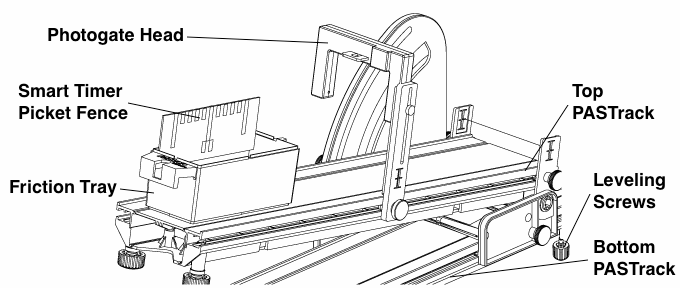
\includegraphics[width=0.9\textwidth]{./Exp3/pic/apparatus.png}
    \end{center}
    \caption{Inclined Plane Apparatus.}
    \label{fig:apparatusplane}
\end{figure}

\begin{enumerate}
    \item Set up the PAStrack and Inclined Plane Accessory as shown in Figure \ref{fig:apparatusplane} with a Photogate Head and Photogate Bracket. Elevate the PAStrack to a shallow angle (a few degrees).
    \item Check if the inclined plane is leveled.  This is done by placing the level across the end of the inclined plane (i.e. perpendicular to the long axis).  See if the bubble in the liquid is inbetween the two lines of the tube.  If not, adjust the levelling screws of the inclined plane until the bubble is centered.
    \item Select a Friction Tray and record its bottom material in Table \ref{planedatatable}. Tape the Smart Timer Picket Fence to the Friction Tray so that the 1 cm `picket fence' pattern is at the top (this is the side with {\it{more}} ticks).
    \item Set the Friction Tray on the PAStrack and adjust the Photogate Head so that the 1 cm `picket fence' pattern of the Smart Timer Picket Fence will interrupt the photogate beam as the Friction Tray moves through the photogate.  Put the Friction Tray at the top of the track where it will be released from rest.
    \item Raise the angle of the the PAStrack so that when the Friction Tray is released from the top, it accelerates down the plane. We recommend using an incline angle less than $15$ degrees. Record the angle in Table \ref{planedatatable}.
    \item Set up the Photogate Head and open the DataStudio file "Inclined Plane."
    \item Start recording data.  Release the Friction Tray from rest.  Stop recording data when the tray reaches the bottom of the track.
    \item Complete three trials of the data recording procedure for the first Friction Tray, recording the acceleration after each run in table \ref{planedatatable} (use the statistics tool in Data Studios to find the average acceleration during the run). Make sure to use the same release position in each trial.
        \item Calculate the average acceleration for the Friction Tray and use the average acceleration and the angle to determine the coefficient of kinetic friction, $\mu_k$ with error due to uncertainty in average acceleration $a_\text{ave}$. You can find the uncertainty in average acceleration by determining the standard deviation. The mathematical expression is repeated below.
\begin{gather}
\sigma = \sqrt{\frac{1}{N}\sum_{i}^{N} (a_i - a_{\text{ave}})^2} 
\end{gather}
Where $a_{avg}$ is the average acceleration you calculated in lab. $N$ is the total number of data points. 
\item  Make sure to record $a_{ave}$ and $\mu_k$ in table \ref{planedatatable}.
     \item The coefficient of friction for such a plastic-on-plastic combination is $0.2-0.4$.  How does this quantitatively compare with your result? Does it agree with error? If not, discuss the largest sources of error in measuring the coefficient of kinetic friction $\mu_k$.
    \item When you are finished taking data, make sure to exit DataStudios and {\bf{\it{do not}}} save your settings.
\end{enumerate}

\begin{table}
\begin{center}
\begin{tabular}{|l |p{5 cm}| p{5 cm} |}
\hline
	Material &  \\
	\hline
	Angle& \\
	\hline
	$a_{trial 1}$& \\
	\hline
	$a_{trail 2}$& \\
	\hline
	$a_{trial 3}$& \\
	\hline
	$a_{average}$& \\
	\hline
	$\mu_k$& \\
	\hline
\end{tabular}
\end{center}
\caption{Inclined Plane Data Table.}
\label{planedatatable}
\end{table}

\section{Lab Preparation Examples}
{\bf{Note: Suggested prelab questions are in bold. These will help will conceptual understanding of the laboratory experiments.}}
\\
\noindent \underline{Vectors}:\myskip

1. Add the following two vectors algebraically:
\begin{equation*}
    \mathbf{u} = (1,2),\quad \mathbf{v} = (2,-5)
\end{equation*}

2. Draw the two vectors described above and add them graphically. \myskip

{\bf{3. Graphically add the two vectors below:}}
\begin{figure}[h]
    \begin{center}
        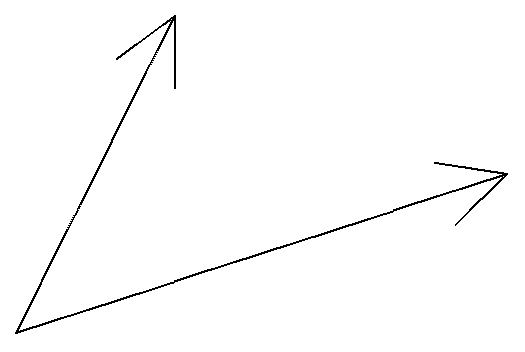
\includegraphics[width=0.3\textwidth]{./Exp3/pic/image4.png}
    \end{center}
\end{figure}

4. Draw the two vectors $\mathbf{u} = (3,-5)$, $\mathbf{v} = (-1,7)$ and graphically check if their sum points in the same direction as the vector $\mathbf{w} = (-1,-1)$.\myskip

5. Split the vectors below into the two given components $(x,y)$ and add them up:
\begin{figure}[h]
    \begin{center}
        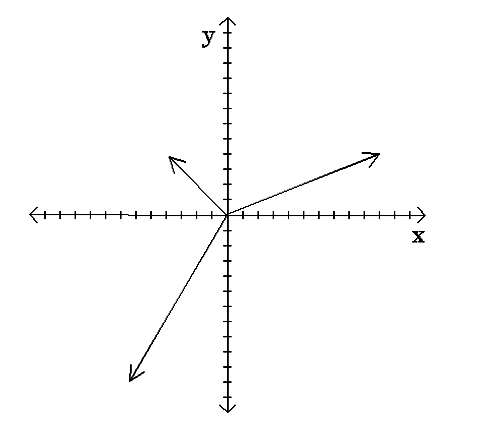
\includegraphics[width=0.4\textwidth]{./Exp3/pic/image5.png}
    \end{center}
\end{figure}

6. Does the sum of the 5 forces $\mathbf{F}_1,\dots,\mathbf{F}_5$ below vanish?
\begin{align*}
    \mathbf{F}_1 &= (1,2,3)\,\mathrm{N},\quad \mathbf{F}_2 = (1,0,-5)\,\mathrm{N},\quad \mathbf{F}_3 = (0,-3,7)\,\mathrm{N}, \\ 
    \mathbf{F}_4 &= (-3,1,0)\,\mathrm{N},\quad \mathbf{F}_5 = (1,0,0)\,\mathrm{N}
\end{align*}

7. Show graphically that the sum of the three vectors $\mathbf{u} = (1,-2)$, $\mathbf{v} = (-3,4)$, $\mathbf{w} = (2,-2)$ vanishes.\myskip

{\bf{8. Does the sum of the following three vectors vanish within uncertainty?}}
\begin{equation*}
    \mathbf{u} = (10 \pm 1, -5 \pm 1),\quad \mathbf{v} = (-13 \pm 1, 7 \pm 1),\quad \mathbf{w} = (7 \pm 1, -3 \pm 1)
\end{equation*}


\noindent \underline{Spring}:\myskip

9. If a spring stretches $5\,\mathrm{cm}$ when you put $100\,\mathrm{g}$ on it, what is the spring constant? \myskip

{\bf{10. If you set a mass of $10.0 \pm 0.1\,\mathrm{g}$ on a spring with spring constant, $k = 5.0 \pm 0.2 \,\mathrm{N/m}$, how long will it stretch?}} \myskip

\noindent \underline{Best-Fit Line}: \myskip

{\bf{11. For the following force versus 1/distance diagram draw in the maximum and minimum slope and the best-fit line.}}
\begin{figure}[h]
    \begin{center}
        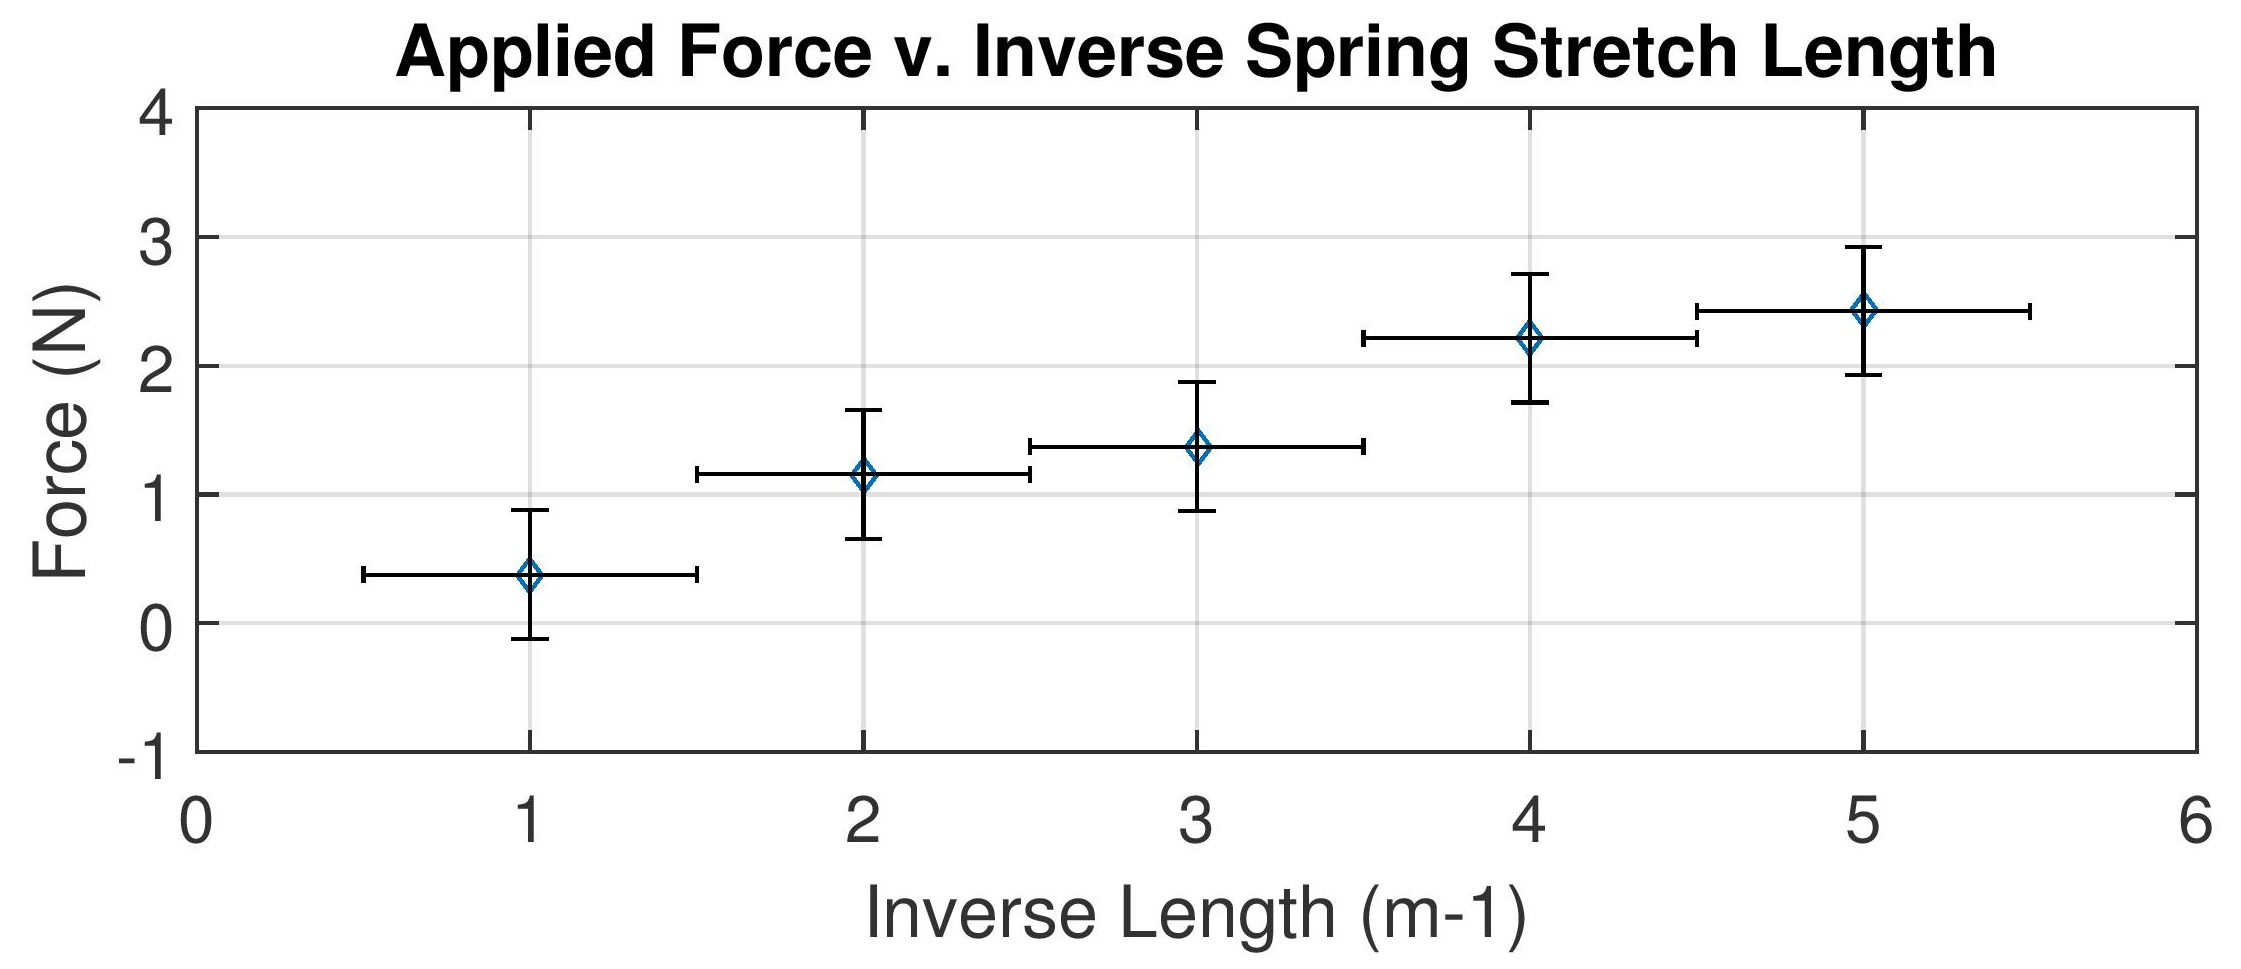
\includegraphics[width=0.9\textwidth]{./Exp3/pic/image15.jpg}
    \end{center}
\end{figure}

12. Fill in the table and draw a force vs. stretch diagram for the following data. Draw the maximum and minimum slope and the best-fit line. Give the value of the spring constant including uncertainty (via maximum and minimum slope curve).
\begin{table}[h]
    \centering
    \begin{tabular}{|l|l|}
        \hline 
        Stretch in $\mathrm{cm}$ & Force in $\mathrm{N}$ \\ \hline
        10 & $1\pm 2$ \\ \hline
        25 & $3\pm 1$ \\ \hline
        50 & $4\pm 2$ \\ \hline
        75 & $8\pm 1$ \\ \hline
        100 & $9\pm 1$ \\ \hline
    \end{tabular}
\end{table}

\noindent \underline{Explanations}:\myskip

13. Explain why a line fit to many measurements gives a better result than a single measurement. \myskip

{\bf{14. Put a string through a book with the binding facing upwards. Try to pull the strings until they are horizontal.  Why is this impossible (your string will usually break)?}}



